% Work-MAT -- 2. rocnik, hodina 02.
% Opakovani uciva prvniho rocniku: myslenkova mapa a priklady.
\documentclass[11pt,a4paper]{article}
\input{../../sablony/pripravy/priprava.sty}
\usepackage{tikz}
\usetikzlibrary{arrows.meta,positioning}
\nastavPripravu{2. ročník}{Funkce}{02}{Opakování funkcí: myšlenková mapa}
\begin{document}
\poznamka{Účel hodiny: diagnostikovat, co žáci opravdu umějí z 1. ročníku, a obnovit základní pojmy bez dlouhého frontálního výkladu. Orientačně: tvorba mapy 12 min, společná kontrola 7 min, dva řešené příklady 13 min, samostatná práce 10 min, závěr 3 min. Příklady s racionální funkcí jsou náročnější rezerva.}

\blok{Společná myšlenková mapa: co všechno víme o funkci?}
Na tabuli napiš doprostřed slovo \emph{funkce} a vyzvi žáky, aby sami navrhli větve mapy. Odlišuj \emph{předpis} od \emph{funkce}: ke konkrétnímu předpisu patří i definiční obor. Pak porovnejte žákovskou mapu s následující oporou.

\begin{center}
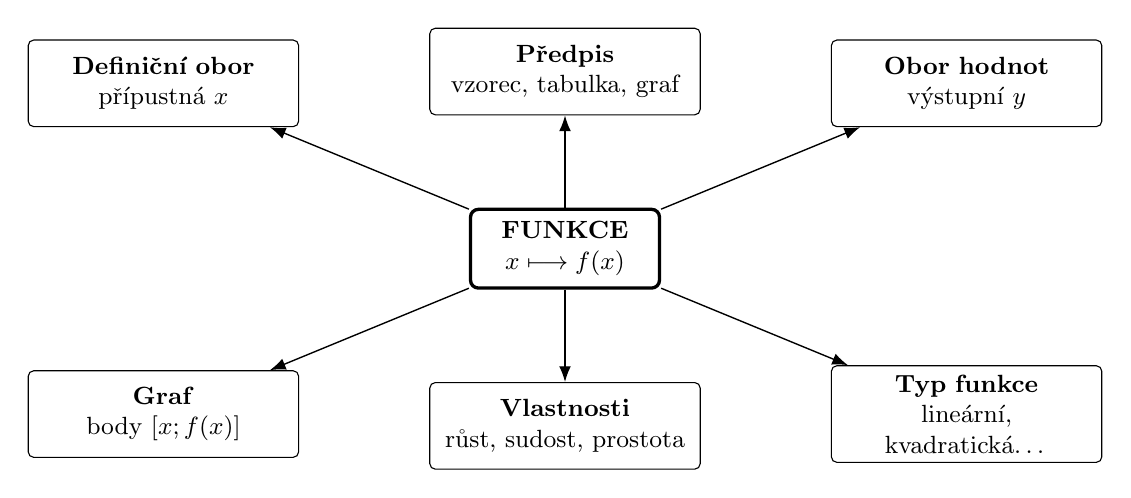
\begin{tikzpicture}[font=\small,>=Latex,
  central/.style={draw,rounded corners=1mm,very thick,align=center,minimum width=24mm,minimum height=10mm},
  leaf/.style={draw,rounded corners=.7mm,align=center,text width=32mm,minimum height=11mm}]
\node[central] (c) at (0,0) {\textbf{FUNKCE}\\$x\longmapsto f(x)$};
\node[leaf] (a) at (-5.1,2.1) {\textbf{Definiční obor}\\přípustná $x$};
\node[leaf] (b) at (0,2.25) {\textbf{Předpis}\\vzorec, tabulka, graf};
\node[leaf] (d) at (5.1,2.1) {\textbf{Obor hodnot}\\výstupní $y$};
\node[leaf] (e) at (-5.1,-2.1) {\textbf{Graf}\\body $[x;f(x)]$};
\node[leaf] (f) at (0,-2.25) {\textbf{Vlastnosti}\\růst, sudost, prostota};
\node[leaf] (g) at (5.1,-2.1) {\textbf{Typ funkce}\\lineární, kvadratická\dots};
\foreach \n in {a,b,d,e,f,g} {\draw[-{Latex[length=2mm]},line width=.5pt] (c)--(\n);}
\end{tikzpicture}
\end{center}

\poznamka{Mapa je kostra, nikoliv hotový zápis ke slepému opsání. Větve doplň slovy žáků: průsečíky s osami, monotonie, omezenost, extrémy, funkce sudá a lichá. Připomeň, že argumenty čteme na vodorovné ose a funkční hodnoty na svislé.}

\blok{Zopakování na jednom grafu a jednom předpisu}
\begin{prikladReseniBox}[title={Příklad 1}]
Je dána funkce $f(x)=x^2-4x+3$ na $\mathbb R$. Urči vrchol, průsečíky s osami, $D(f)$, $H(f)$ a intervaly monotónnosti. Nakresli náčrtek.
\tcblower
Doplněním na čtverec dostaneme $f(x)=(x-2)^2-1$. Vrchol je $V=[2;-1]$ a osa souměrnosti $x=2$. Rovnice $f(x)=0$ má kořeny $x=1$ a $x=3$; s osou $y$ se graf protíná v $[0;3]$. Platí $D(f)=\mathbb R$, $H(f)=\langle-1;+\infty)$, funkce klesá na $(-\infty;2\rangle$ a roste na $\langle2;+\infty)$. Minimum $-1$ nastává pro $x=2$.
\end{prikladReseniBox}
\poznamka{Nech žáky zdůvodnit, proč se obor hodnot mění po svislém posunu paraboly. Kontrolní otázka: je tato funkce na $\mathbb R$ prostá? Není, protože $f(1)=f(3)=0$.}

\begin{prikladReseniBox}[title={Příklad 2}]
Funkce $g(x)=\frac{2x+1}{x-3}$ má definiční obor $\mathbb R\setminus\{3\}$. Urči $g(0)$, řešení rovnice $g(x)=0$ a obor hodnot.
\tcblower
$g(0)=-\frac13$. Zlomek je roven nule právě tehdy, když $2x+1=0$ a jmenovatel není nulový; proto $x=-\frac12$. Pro obor hodnot řešíme $y=\frac{2x+1}{x-3}$:
\[
y(x-3)=2x+1\quad\Longrightarrow\quad x=\frac{3y+1}{y-2}.
\]
Tento postup funguje pro všechna $y\ne2$, zatímco $y=2$ by vedlo na spor $1=-6$. Tedy $H(g)=\mathbb R\setminus\{2\}$.
\end{prikladReseniBox}
\poznamka{Příklad 2 je určen zejména rychlejším žákům; při časové tísni stačí $D(g)$, $g(0)$ a nulový bod. Obor hodnot lze vynechat nebo doplnit příště.}

\blok{Samostatná práce}
\begin{zadaniReseniBox}[title={Samostatná práce 1}]
\begin{enumerate}[label=\alph*)]
\item Pro $h(x)=-2x+6$ urči průsečíky s osami a rozhodni o monotónnosti.
\item Pro $p(x)=|x-1|$ urči $D(p)$, $H(p)$, minimum a kde nastává.
\item U $q(x)=\sqrt{x+2}$ urči $D(q)$, $H(q)$ a $q(7)$.
\item Rozhodni, zda je $r(x)=x^2$ na $\mathbb R$ prostá. Uveď dvojici argumentů jako důkaz.
\end{enumerate}
\tcblower
\begin{enumerate}[label=\alph*)]
\item S osou $y$: $[0;6]$; s osou $x$: $[3;0]$. Funkce je klesající.
\item $D(p)=\mathbb R$, $H(p)=\langle0;+\infty)$, minimum $0$ pro $x=1$.
\item $D(q)=\langle-2;+\infty)$, $H(q)=\langle0;+\infty)$, $q(7)=3$.
\item Není prostá, například $r(-2)=r(2)=4$ při $-2\ne2$.
\end{enumerate}
\end{zadaniReseniBox}

\begin{zadaniReseniBox}[title={Rozšíření 1}]
Sestav vlastní myšlenkovou mapu \emph{lineární versus kvadratická funkce}: porovnej graf, počet nulových bodů, monotónnost a možné obory hodnot.
\tcblower
Lineární funkce s nenulovou směrnicí má graf přímky, jediný nulový bod, je na $\mathbb R$ přísně monotónní a má obor hodnot $\mathbb R$. Kvadratická funkce s nenulovým koeficientem u $x^2$ má graf paraboly, může mít $0$, $1$ nebo $2$ nulové body, na celé $\mathbb R$ není monotónní a její obor hodnot je podle orientace paraboly polopřímka.
\end{zadaniReseniBox}

\blok{Závěr a most k nové látce}
Polož otázku: \emph{Kdy lze z hodnoty $y$ jednoznačně určit původní argument $x$?} Pro $f(x)=3x-1$ ano; pro $x^2$ na celém $\mathbb R$ nikoli. Právě to bude jádrem příští hodiny.

\begin{zadaniReseniBox}[title={Domácí úkol}]
\begin{enumerate}[label=\alph*)]
\item Urči $D(f)$, $H(f)$ a vrchol $f(x)=(x+1)^2-4$.
\item Pro $g(x)=\frac1{x+2}$ napiš definiční obor a vypočítej $g(-1)$.
\item Připrav dvě vlastní věty vysvětlující rozdíl mezi \emph{definičním oborem} a \emph{oborem hodnot}.
\item Urči definiční obor a obor hodnot $h(x)=\frac{3}{x-1}$.
\item Načrtni $p(x)=|x-2|-1$ a urči minimum.
\end{enumerate}
\tcblower
\begin{enumerate}[label=\alph*)]
\item $D(f)=\mathbb R$, $H(f)=\langle-4;+\infty)$, $V=[-1;-4]$.
\item $D(g)=\mathbb R\setminus\{-2\}$, $g(-1)=1$.
\item Například: definiční obor je množina přípustných vstupů $x$; obor hodnot je množina skutečně dosažených výstupů $f(x)$.
\item $D(h)=\mathbb R\setminus\{1\}$, $H(h)=\mathbb R\setminus\{0\}$.
\item Vrchol $[2;-1]$, minimum $-1$, $H(p)=\langle-1;\infty)$.
\end{enumerate}
\end{zadaniReseniBox}
\end{document}
